\section{Theoretical Basics}
\subsection{Basics of Tumor Biology}
\begin{figure}[h]
    \centering
    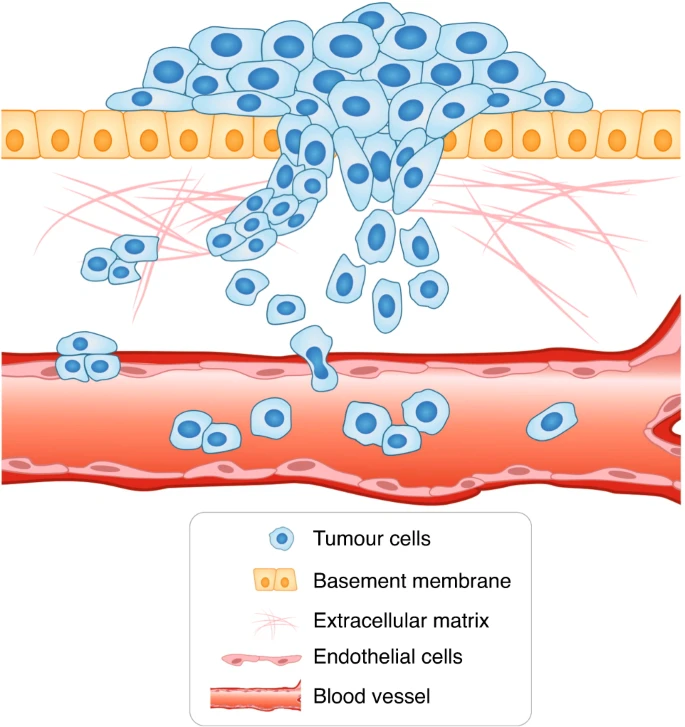
\includegraphics[width=0.85\textwidth]{resources/images/tumour_invasion_stage.png}
    \caption{Tumor Invasion Stage}
    \label{fig:tumour_invasion_stage}
\end{figure}

The body of a living creature is made up of more than 200 different types of cells, the coordination between the cells and their surroundings keep the body running. Each of these cells is built from the genetic information encoded in the DNA, located in the cells' nuclei. Though the nucleotide sequence of DNA is well checked and maintained throughout the cell's life, mutations still occur that cause the changes in the DNA of a cell. These mutations may be of a positive, negative or neutral nature. In the case of a negative mutation this alternation of the DNA may cause diseases, with cancer being one of them. The failure of the complex system managing cell birth, proliferation, and cell death (apoptosis) causes cancer, resulting in an uncontrolled cell proliferation in a at first local area. A conglomeration of cancer cells is called a tumor. \newline
Cancer diseases can be categorized medically into five stages. First the tumor initiation phase where it comes to the above explained genetic mutations of normal cells. The next stage is the tumor promotion stage, in which the mutated cells of phase one may experience further genetic alterations, with the result of uncontrolled growth and proliferation of the cancerous cells. The third stage is the tumor progression stage, where the cancerous cells progress in growing and proliferating, reaching a critical mass, they form a tumor at a local site of the body. Fourth comes the invasion stage, which is shown in figure~\ref{fig:tumour_invasion_stage}. Here the tumor is able to invade surrouding tissue by breaking through the cellular membrane, invading the extracellular matrix inside and entering the blood circulation system or the lymphatic system. Next the tumor cells which have invaded the blood circulation of lymphatic system spread throughout the body and form new tumors. This stage is called Metastization. To further grow the tumors need to have access to nutrient and oxygen supply. During angiogensis a tumor develops blood vessels of its own securing its nutritional provision. At this stage first symptoms of host may appear, enabling medical treatment.\newline
In our model the focus lies on the first two stages; tumor invasion and tumor progression. The tumor invasion stage is characterized by the malignant cells gaining the ability to penetrate and invade the surrouding tissue. The tumor cells break through the normal tissue barrier and infiltrate neighboring structures. In order to do so the cancer cells produce so called matrix-degrading enzymes which break down the extracellular matrix. This not only helps local spreading, but also destroys otherwise healthy tissue and cells in the affected area. In the next phase the tumor progression stage, the tumor has grown larger and the cancerous cells take on more aggressive behaviour, by invading the surrounding area further. Whilst they keep growing uncontrolled they are also affected by further genetic instabilities, which lead to more mutations, resulting possibly in the development of resistence mechanisms against for example degrading factors. Already in this stage the affected area is exposed to heavy tissue damage and functional disabilities.\newline
The most important factors influencing those two phases are the genetic dispositions of the tumor cells towards proliferation and the evasion of apoptosis, programmed cell death, which increase the invasive potential. Another important factor is the geometry of the extracellular matrix, as well as the exact macromolcules which make it up. A strong immune biological defense reaction also helps the body defend against the spreading of the cancer cells, so evasion of detection and destruction of the tumor cells plays a key role for the first stages. To invade the affected area the malignant cells need to be able to move freely and fastly. In order to do so cancer cells can gain the ability to lose adhesion properties which healthy cells normally have, to allow migrating into surrouding tissue. 
Another organization principle can be found in the Hallmarks of cancer of Douglas Hanahan and Robert Weinberg~\cite{10.1158/2159-8290.CD-21-1059}. They describe a set of functional capabilities, eight hallmark capabilities and two enabling characteristics, that are commonly acquired by cancer cells and contribute to their ability to grow uncontrollably, evade the immune system, and metastasize. These hallmarks: sustaining proliferative signaling, evading growth suppressors, avoiding immune destruction, enabling replicative immortality, tumor-promoting inflammation, activating invasion and metastasation, inducing or accessing vasculature, genome instability and mutation, resisting cell death deregulating cellular metabolism. These Hallmarks of Cancer toghether contribute to the development and progression of cancer and provide targets for therapeutic intervention and research efforts aimed at understanding and treating the disease. 
In our model we see many of the capabilities incorporated. Proliferative signalling only relies on the tumor cells themselves and not of typically other hormones or molecules, allowing them to proliferate rapidly without external growth signals. The immmune destruction and induced cell death are avoided, optimizing them to survive and accumulate genetic mutations that promote tumor growth. The tumor cells are capable of invading the surrounding tissue, modelled by the extracellular matrix.

\subsection{Mathematical Methods in Oncology}
Mathematical methods and models in Oncology play a crucial role in analysing, understanding and predicting cancer development. Since the obejctive of this research underlies complex and intricate biochemical systems and mechanisms, there exist many models, which find their respective application in distinct areas of this research field. These methods can be coarsely divided into three sections; continuous, discrete and hybrid models~\cite{BEKISZ2020101198}. For describing tumor growth, exponential and logisitc growth models are often used, the later allowing limiting factors to play a role during modelling. These methods are a subclass of the differential equations approach which base their functionality on an ordinary or partial differential equation, studying the continuous approach. Like in our model they are not limited to consist of only one equation but can of many, incorporating systematic dependencies on other factors. These models in general deal with continuous quantities like densities, or concentrations, for example spacial and temporal nutritional supply or drug concentration, as well as their effects on the affected area over time. Discrete models use discrete entities to describe the behaviour of tumour cells and their interactions with surrouding tissue. They allow to model a wide range of biological and chemical processes which are hard to describe continuously. Common used types in mathematical oncology are for example Cellular Automata or Agent-Based Models. Cellular Automata represent cells as entities with states on a grid, with each cell being allowed to change states according to a set of rules based on its own current state and the states of the neighbors, whereas Agent-Based Models enable a differentiation of types of cells and allow movement that is not restricted to a grid implementing complex mechanics on cell-cell or cell-environment levels. Using these discrete models allows researchers to focus on biological effects during modelling, which are hard to describe in continuous models. With these approaches we can also simulate genetic and evolutionary events. For example studying the genetic alternations of tumor cells or the interaction between healthy and cancerous cells.\newline 
Hybrid models combine both aforementioned methods, of using both continuous and discrete approachese. Like in the model proposed by Franssen et al.~\cite{franssen_mathematical_2019} or Anderson et al.~\cite{anderson_continuous_1998}, these approaches allow to incorporate the exactness of continuous models with a wide range of biological effects described by discrete models. \newline
But not all models try to model tumor growth, there are others concerning for example optimality regarding drug dosages or radiation exposition, offering personalized treatment, or Machine Learining and Data Mining methods analysing large datasets, to identify patters and predict outcomes. The later method may be used in all kinds of applications, for example spacial or temporal cancer development but also for drug dosage optimization for individual patients. Putting all these methods together gives us an powerful toolbox to simulate and understand cancer biology. Like the last years have shown they are applied in a wide range, offering insight for all areas of cancer research. Therefore it is important not only to come up with methods but to also evaluate their usefulness and meaningfulness regarding different areas of research.